\documentclass[conference]{IEEEtran}
\usepackage{amsmath,amssymb,graphicx,booktabs}
\pagestyle{empty}
\renewcommand{\thefigure}{S\arabic{figure}}
\renewcommand{\thetable}{S\arabic{table}}
\begin{document}
\onecolumn
\begin{center}{\Large\bfseries Supplementary evidence: computational compatibility}\end{center}
\noindent This companion preserves the complete development-pilot RMS table and visualizes the measured bridge between the archived computation $G$ and native pilot computation $G^\star$. Both use the same eight saved development snapshots: two tasks, four initialization clusters, and queries 11/22 within each cluster. These are dependent exploratory observations, not new task-held-out evidence.

\begin{figure}[!h]
\centering
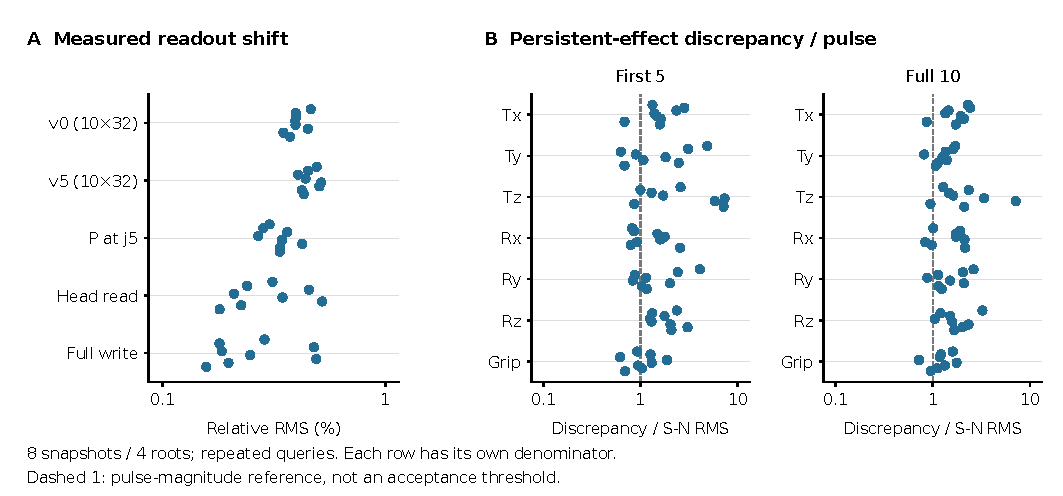
\includegraphics[width=180mm]{figures/F1-BRIDGE-ERROR.pdf}
\caption{\textbf{Similar read proxies do not establish interchangeable effect targets.}
\textbf{A:} each point reports the old/new discrepancy RMS divided by that field's own old-reference RMS, in percent. The vector fields $v_0,v_5$ use the complete native $10\times32$ tensors, including non-adapter coordinates; attention probabilities and the two FP64 algebraic read/write proxies have their own tensor denominators. These proxies are not native BF16 intervention writes.
\textbf{B:} for each controller-input coordinate, points show
$\mathrm{RMS}[(P^\star-N^\star)-(P-N)]/\mathrm{RMS}[S^\star-N^\star]$,
where each persistent effect uses its own none baseline and starred endpoints use $G^\star$. First-five and full-ten windows retain all eight snapshots. Vertical offsets encode fixed snapshot order, not uncertainty. The line at one is a signal-magnitude reference, not an equivalence, physical, or significance threshold. Panels have different denominators and do not measure a causal amplification factor. Full support and the alternative $S^\star-R^\star$ denominator are retained in the accompanying table archive.}
\end{figure}

\noindent\textbf{Interpretation.} Historical feature/target reconstruction passes all 40 exact checks, but the two computations differ in unedited T vector fields, measured attention probabilities and both algebraic proxies. Their own-baseline persistent effects differ in all 112 dependent coordinate--window cells. This audit does not explain earlier cross-task prediction errors, identify a unique numerical cause, or invalidate the internally qualified $G^\star$ S/R/P comparisons. Fresh clean-C flow and cross-graph physical effects remain unmeasured. Four separately reduced RMS pairs differ by one floating-point interval despite identical payloads; their original scalar values are retained, without changing exact array identities or strict ratio classifications.

\begin{table}[!h]
\centering
\caption{Development pilot: median first-five RMS over eight fixed snapshots. Entries report RMS divided by $10^{-4}$, separately in each coordinate's controller-input units; no cross-axis norm or physical-motion claim.}
\label{tab:pulse}
\begin{tabular}{@{}lrrr@{}}\toprule
Command coordinate & $S-N$ & $R-N$ & $S-R$\\\midrule
Translation x & 5.05 & 5.20 & 7.51\\
Translation y & 3.61 & 5.65 & 4.21\\
Translation z & 4.15 & 5.06 & 5.48\\
Rotation x & 0.78 & 0.62 & 0.45\\
Rotation y & 1.17 & 0.80 & 1.11\\
Rotation z & 1.39 & 0.97 & 1.45\\
Gripper & 10.40 & 7.21 & 11.15\\
\bottomrule
\end{tabular}
\end{table}


\noindent\textbf{Complete support.} The source bundle includes all 1,000 comparison rows, per-coordinate descriptive summaries, undefined/zero cases, near-one display-sensitivity records, numerical identities, and the preserved technical failures. No new model call, fit, training, or environment step was used for this bridge or its figure.
\clearpage
\begin{center}{\Large\bfseries Supplementary evidence: native-write calibration}\end{center}
\noindent At the first intervention site ($j5$, layer~9), this audit compares S--N and R--N on the same eight saved snapshots: two tasks, four initialization clusters, and two queries per cluster. Twelve recorded pre-site fields agree exactly for every pair (192 checks); these are dependent qualification comparisons. The original S/R content increments are nearly norm-matched, not exactly matched. Table~S2 retains every full-ten pair without filtering.

\noindent Let $\Delta O_a=O_a-O_N$ be the difference between captured native pre-gate attention outputs, and $\Delta H_a=H_a-H_N$ the difference after attention-residual addition, for $a\in\{S,R\}$. The shared pre-site state and gate make these paired quantities well defined. The algebraic quantities are
\[
 \widehat{\Delta O}_a=\sum_h(P_hE_a)W_h^O,\qquad
 \widetilde w_a=\operatorname{fl}_{64}\!\left(g\odot\widehat{\Delta O}_a\right).
\]
All full-ten vectors contain $10\times1024$ coordinates. Captured BF16 values are decoded for comparison; the proxy is evaluated in FP64 and is not a native intervention write. The table reports
\[
 e_O=100\frac{\|\widehat{\Delta O}_a-\Delta O_a\|_F}{\|\Delta O_a\|_F},
 \qquad
 e_H=100\frac{\|\widetilde w_a-\Delta H_a\|_F}{\|\Delta H_a\|_F},
 \qquad
 d_{S/R}=\frac{\|\Delta H_S\|_F}{\|\Delta H_R\|_F}.
\]
The cosine columns are $\cos(\widetilde w_a,\Delta H_a)$; they are not S/R cosines or prediction scores. All error and dose denominators are defined native norms.

\begin{table}[!h]
\centering
\caption{Native-write calibration at $j5$/layer~9. Full-ten values retain all eight snapshots and both S--N/R--N pairs. Dose is the native $\Delta H$ norm ratio S/R. Error columns divide proxy error norm by the corresponding native difference norm; cosine compares the gated proxy with native $\Delta H$.}
\label{tab:native-fidelity}
\setlength{\tabcolsep}{5pt}
\renewcommand{\arraystretch}{1.15}
\begin{tabular}{@{}lrrrrrrr@{}}\toprule
Snapshot & Native dose & \multicolumn{2}{c}{Pre-gate error (\%)} & \multicolumn{2}{c}{Gated error (\%)} & \multicolumn{2}{c}{Gated cosine}\\
 & S/R & S & R & S & R & S & R\\\midrule
T00/R00, q11 & 1.331 & 1.46 & 1.82 & 16.52 & 11.13 & 0.986302 & 0.993792\\
T00/R00, q22 & 2.352 & 1.30 & 2.89 & 9.63 & 21.79 & 0.995430 & 0.976013\\
T00/R01, q11 & 1.621 & 3.13 & 4.86 & 21.85 & 26.48 & 0.975908 & 0.964370\\
T00/R01, q22 & 1.798 & 1.36 & 2.25 & 10.67 & 19.27 & 0.994291 & 0.981253\\
T01/R00, q11 & 1.341 & 5.57 & 7.02 & 50.12 & 57.49 & 0.866936 & 0.818276\\
T01/R00, q22 & 1.319 & 2.49 & 3.16 & 18.80 & 26.77 & 0.982181 & 0.963514\\
T01/R01, q11 & 1.463 & 3.50 & 4.70 & 32.30 & 21.24 & 0.946858 & 0.977186\\
T01/R01, q22 & 1.944 & 1.31 & 2.31 & 16.16 & 17.22 & 0.986863 & 0.985068\\
\bottomrule
\end{tabular}
\end{table}


\noindent\textbf{Magnitude and zero support.} The best full-ten gated case, T00/R00/q22 S--N, has 9.63\% relative error and cosine 0.995430, so the proxy is not uniformly poor. Conversely, T01/R00/q11 R--N has 57.49\% error and cosine 0.818276. In that case, 6696 of 6711 jointly nonzero coordinates agree in sign, while another 3529 of 10240 coordinates are native-zero/proxy-nonzero. Conditional sign agreement therefore does not establish full-coordinate fidelity. At its single position $p=0$, error reaches 88.43\% and cosine is 0.490452 over 1024 coordinates; this position-level maximum is not a full-ten result.

\noindent\textbf{Accounting boundary.} With the recorded gate and pre-state fixed, saved-value algebra gives
\[
 g\odot\widehat{\Delta O}-\Delta H
 =\underbrace{g\odot(\widehat{\Delta O}-\Delta O)}_{\epsilon_{\rm proj}}
 +\underbrace{g\odot\Delta O-\Delta H}_{\epsilon_{\rm gr}}.
\]
This identity uses exact products of the saved factors; the fidelity columns use rounded FP64 products, whose last bits are not assumed identical. The combined gate/residual term is larger in norm in the saved decomposition, but the energy identity retains $2\langle\epsilon_{\rm proj},\epsilon_{\rm gr}\rangle$, with both positive and negative cases. These are not causal variance shares. No intermediate native gated product was captured, so multiplication and residual-addition effects are not separated; exact closure does not prove a native-kernel mechanism.

\noindent\textbf{Scope and full support.} Native-dose differences may be intermediaries of the valid near-equal-E total-effect comparison; matching native writes would change the question. This calibration explains neither the historical task-transfer errors nor the old/new execution difference, and supplies no physical-motion or task-success evidence. Best-scalar projections in the accompanying data are target-visible oracle geometry, not predictions. The original \texttt{WRITE-FIDELITY.json.gz}, \texttt{DECOMPOSITION.json.gz}, \texttt{DOSE-AND-ENDPOINTS.json} and \texttt{STATE-CHECKS.json} retain first-five, full-ten and all-position support, including S--R, zero cases and every counterexample.
\clearpage
\begin{center}{\Large\bfseries Supplementary evidence: command-interface mapping}\end{center}
\noindent The 24 cached N/S/R chunks use the same eight development snapshots as Tables~S1--S2: two tasks, four initialization clusters, and queries 11/22. A source-based CPU diagnostic applies the recorded controller configuration to each command, without importing the controller or executing an environment. The first five positions are the intended execution prefix; the full ten are retained as a dependent secondary window. Neither window was executed by this diagnostic.

\noindent\textbf{Map and units.} The source-bound setup selects OSC\_POSE with fixed impedance, delta control and no interpolation, together with PandaGripper on OnTheGroundPanda. For an unnormalized seven-component controller input $a$, the arm map is
\[
 c_i=\operatorname{clip}(a_i,-1,1),\qquad
 d_i=(c_i-0)s_i+0,\qquad
 s=(0.05,0.05,0.05,0.5,0.5,0.5).
\]
The written operation order is retained in FP64. These are controller goal increments, not measured displacement. The seventh component is reduced to $z=\operatorname{sign}(a_7)\in\{-1,0,1\}$. Numeric and bitwise equality, signed zero, clipping, and scaling-rounding effects are recorded separately. No tolerance defines an unequal command.

\begin{table}[!h]
\centering
\caption{Source-defined command-interface mapping. Counts are unequal positions among the eight fixed snapshots. All three contrasts are retained. Raw and mapped are numeric comparisons; mapped gripper values are sign symbols, not actuator targets. First-five/full-ten denominators are 40/80 dependent positions.}
\label{tab:control-map}
\begin{tabular}{@{}llrrr@{}}\toprule
Gripper contrast & Window & Raw unequal & Sign unequal & Comparisons\\\midrule
S--N & First 5 & 28 & 0 & 40\\
S--N & Full 10 & 57 & 0 & 80\\
R--N & First 5 & 28 & 0 & 40\\
R--N & Full 10 & 54 & 0 & 80\\
S--R & First 5 & 29 & 0 & 40\\
S--R & Full 10 & 54 & 0 & 80\\
\bottomrule\end{tabular}
\medskip
\begin{tabular}{@{}lrrrrrr@{}}\toprule
Arm coordinate & \multicolumn{3}{c}{First 5: raw / mapped unequal} & \multicolumn{3}{c}{Full 10: raw / mapped unequal}\\
 & S--N & R--N & S--R & S--N & R--N & S--R\\\midrule
Translation x & 27 / 27 & 30 / 30 & 36 / 36 & 51 / 51 & 57 / 57 & 60 / 60\\
Translation y & 32 / 32 & 33 / 33 & 31 / 31 & 65 / 65 & 65 / 65 & 61 / 61\\
Translation z & 24 / 24 & 27 / 27 & 28 / 28 & 51 / 51 & 50 / 50 & 59 / 59\\
Rotation x & 35 / 35 & 28 / 28 & 30 / 30 & 64 / 64 & 55 / 55 & 59 / 59\\
Rotation y & 34 / 34 & 20 / 20 & 32 / 32 & 65 / 65 & 46 / 46 & 58 / 58\\
Rotation z & 31 / 31 & 28 / 28 & 29 / 29 & 58 / 58 & 53 / 53 & 58 / 58\\
\bottomrule\end{tabular}
\end{table}


\noindent\textbf{Observed boundary.} Every first-five/full-ten gripper pair has the same nonzero sign for all three contrasts. The nonzero raw gripper differences in the table therefore disappear at this sign interface. Conversely, every nonzero arm difference survives the tested clipping/scaling map; no arm difference is erased at clipping or solely by scale rounding. All 24 snapshot--contrast first-five windows retain an arm difference, as do their full-ten counterparts. The retained zero raw differences remain zeros; no case or coordinate is filtered out.

\noindent\textbf{Stateful interpretation.} The actual gripper formatter updates
\[
 c^{g}_{k+1}=\operatorname{clip}\!\left(c^{g}_k+[-1,+1]\,0.01\,z,-1,1\right)
\]
on each internal control update, then rescales it to the compiled actuator range. The audit does not know or simulate $c^{g}_0$. Equal sign sequences imply equal gripper actuator-target sequences only with equal initial gripper memory and update counts. Different arm motion can still change finger motion or contact. Surviving arm goal differences do not establish different torques or end-effector motion: OSC feedback, torque limits and physical dynamics remain unmeasured.

\noindent\textbf{Complete support.} \texttt{POINTS.json.gz} retains all 1,680 axis--position comparisons (240 seven-axis position contrasts); \texttt{WINDOWS.json} retains all 336 axis--window comparisons (48 windows). \texttt{SUMMARY.json} and \texttt{QA.json} preserve source identities, all four root configuration bindings and every case. Counts describe dependent fixed-pilot support, not independent replications or significance. This result establishes a command-interface boundary, not a physical null, task outcome, transfer guarantee, or evidence that full signed representations lack information.
\clearpage
\begin{center}{\Large\bfseries Supplementary evidence: bounded simulator continuation}\end{center}
\noindent This extension tests one fixed development state, T00/R00/q11, chosen for a previously recorded CPU replay witness rather than response magnitude. It executes the first five saved $G^\star$ N/S/R commands at 20~Hz (0.25~s); it adds no neural call, policy feedback or independent task/initialization. The historical parent policy's actually issued commands reconstruct the state and qualify its next five transitions. They are not substituted for the cached diagnostic N baseline.

\noindent\textbf{Paired start and repeat control.} Each branch independently rebuilds the original initialization, executes ten settling steps and replays the same 55 parent commands. The new N-repeat, S and R starts match the recorded declared-state fingerprint, critical controller/gripper/compiled-model state, and pre-command physics/time/pose identity. Before S/R, N-repeat exactly reproduces the retained full five-step N trajectory, including before/after states, returned physical observations, actuator targets, contacts and terminal flags. This is a technical control, not an additional statistical sample.

\noindent The original source qualification and N observations are retained without repeating either case. N originally failed only while closing an auxiliary recorder window after all five commands were observed; that failure remains labeled failed. A separate archived-data check revalidates the source/N records, and the cross-run N repeat gates their use here. The original 13-query sensor schedule, including q12 arming during the final command, remains unchanged. Only post-action recorder closure differs; q12 is left unread in the cached branches. Historical strict image-replay failures remain distinct from this physical-continuation qualification.

\begin{table}[!h]
\centering
\caption{All five observed times, both pulse-versus-none contrasts, at T00/R00/q11. Slot $k$ occurs $0.05k$~s after the matched start. Position and orientation distances are converted from stored metres/radians; the two joint differences keep native qpos units. Contact counts are arm / N. These are ten dependent observations of one state.}
\label{tab:physical-all}
\begin{tabular}{@{}llrrrrc@{}}\toprule
Contrast & Slot & EEF distance ($\mu$m) & Orientation ($\mu$rad) & Finger 1 $\Delta q$ & Finger 2 $\Delta q$ & Contacts\\\midrule
S--N & 1 & 3.713867 & 13.491486 & 5.373847e-10 & 5.198006e-10 & 29 / 29\\
S--N & 2 & 5.193931 & 21.337936 & 9.925756e-09 & 9.876879e-09 & 28 / 28\\
S--N & 3 & 7.132358 & 29.886958 & 5.535649e-09 & 5.476670e-09 & 27 / 27\\
S--N & 4 & 6.920504 & 30.428232 & 4.058385e-10 & -2.900196e-08 & 27 / 27\\
S--N & 5 & 7.652770 & 32.167875 & -8.697751e-07 & -3.111940e-08 & 27 / 27\\
R--N & 1 & 3.509473 & 3.105960 & 6.351180e-09 & 6.342734e-09 & 29 / 29\\
R--N & 2 & 10.566854 & 2.977712 & -7.904187e-09 & -7.910970e-09 & 28 / 28\\
R--N & 3 & 21.047644 & 7.942277 & -2.322729e-09 & -2.319153e-09 & 27 / 27\\
R--N & 4 & 30.742938 & 15.344140 & -8.134126e-09 & -1.089838e-07 & 27 / 27\\
R--N & 5 & 35.743309 & 18.386062 & -5.495644e-06 & -1.446372e-07 & 28 / 27\\
\bottomrule
\end{tabular}
\end{table}


\noindent\textbf{Actuator targets and motion are different observables.} All ten S--N/R--N gripper actuator-target comparisons are equal, but neither two-finger qpos-difference sequence is identically zero. Equal direct targets therefore do not imply equal finger motion under different arm commands. The last R command also has 28 contacts versus N's 27. This does not isolate a contact-mediated mechanism, identify the contacted task object, measure contact force, or demonstrate improvement.

\noindent\textbf{Scale, ranking and negative cases.} S--N position distance decreases at the fourth time (7.132358 to 6.920504~$\mu$m); its trajectory is not monotonically increasing. R has the larger final translation distance, while S has the larger final orientation distance. Larger is not better. All observed N/S/R steps have \texttt{done=false} and \texttt{success=false}; absence of completion in this short window is not a full-task failure. These small, nonzero simulator differences establish local observability, not a practically important effect or statistical significance.

\noindent\textbf{Evidence scope.} The three new branches use 210 environment steps; the retained source/N pair used 140, for 350 cumulative. Native-call limits, source identities, full trajectories, event records, failures and release records remain in the immutable evidence archive. The complete pairwise scalar table and figure preserve all five times; no unobserved tail is padded. The prior tables describe separate retrospective and source-algebra diagnostics. This physical result does not explain their prediction errors, establish same-write-dose mediation, or justify task-transfer or success-rate claims.

\clearpage
\begin{center}{\Large\bfseries Supplementary evidence: complete physical contrasts}\end{center}
\noindent All five timepoints and all three pairwise contrasts are retained below. S--R is derived from the same S and R trajectories as Table~S4. The N repeat is a technical control, not an additional initialization.
\par\medskip\noindent\begin{minipage}{\textwidth}
\makeatletter\def\@captype{figure}\makeatother
\centering
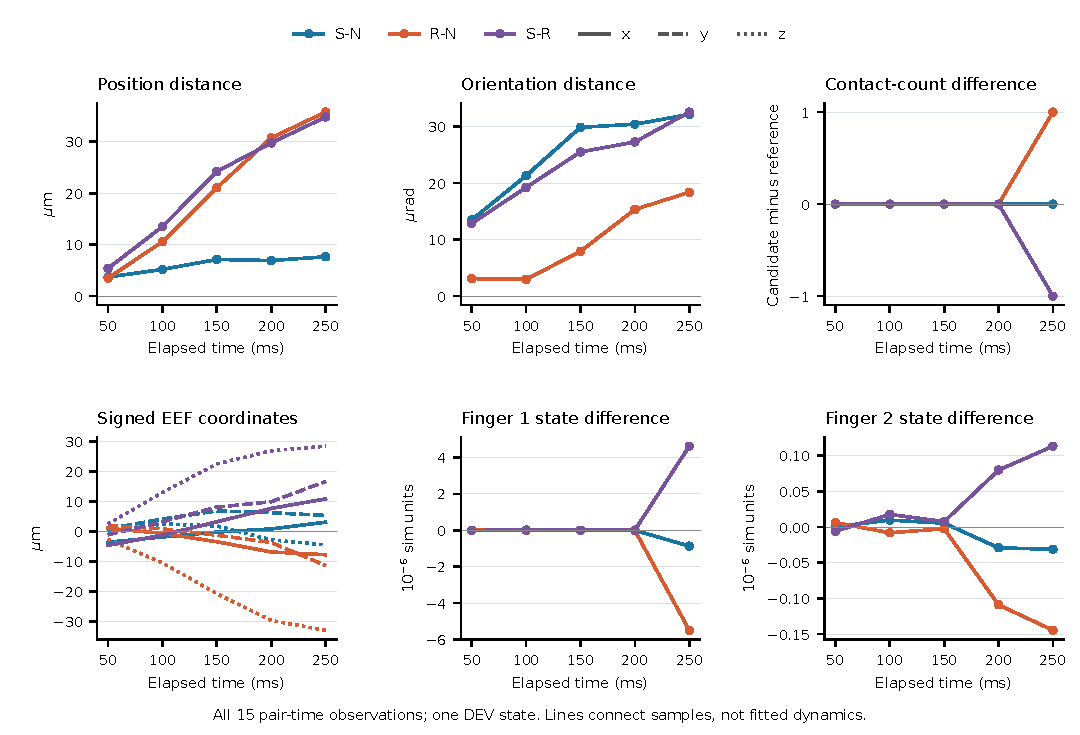
\includegraphics[width=\textwidth]{figures/fig_physical_support.pdf}
\caption{\textbf{No uniform physical ranking.} Three pairwise position/orientation distances and contact-count differences, signed end-effector coordinates, and both signed finger-joint differences. Position is in micrometres; orientation is in microradians; joint differences retain simulator units. All direct gripper actuator targets agree. Lines connect measured samples, not fitted dynamics. All panels refer to one initialization/state; no confidence interval or task-success rate is estimated.}
\end{minipage}\par\medskip
\par\medskip\noindent\begin{minipage}{\textwidth}
\makeatletter\def\@captype{table}\makeatother
\centering
\caption{Shared minus random at all five times. Together with Table~S4, these are all 15 pair--time observations of the same three trajectories, not 15 independent samples. Joint differences retain simulator units; contacts are S / R.}
\label{tab:physical-SR}
\begin{tabular}{@{}lrrrrc@{}}\toprule
Slot & EEF distance ($\mu$m) & Orientation ($\mu$rad) & Finger 1 $\Delta q$ & Finger 2 $\Delta q$ & Contacts\\\midrule
1 & 5.396271 & 12.876368 & -5.813795e-09 & -5.822933e-09 & 29 / 29\\
2 & 13.509382 & 19.241863 & 1.782994e-08 & 1.778785e-08 & 28 / 28\\
3 & 24.207425 & 25.529912 & 7.858378e-09 & 7.795823e-09 & 27 / 27\\
4 & 29.745598 & 27.291051 & 8.539964e-09 & 7.998183e-08 & 27 / 27\\
5 & 34.779465 & 32.575053 & 4.625869e-06 & 1.135178e-07 & 27 / 28\\
\bottomrule
\end{tabular}
\end{minipage}\par\medskip

\noindent\textbf{Complete numerical support.} The evidence bundle includes all 15 scalar/vector records and the executed cloud readout, plus the immutable trajectory references. Exact repeat agreement does not establish robustness to solver settings, independent initializations or longer horizons. Contact counts alone identify neither task objects nor a causal path to joint motion. The short-window differences do not establish practical significance or task benefit.

\end{document}
